\documentclass[10pt,a4paper]{article}

\usepackage[utf8]{inputenc}
\usepackage[T1]{fontenc}
\usepackage[brazil]{babel}
\usepackage{lmodern}
\usepackage{geometry}
\geometry{
	top=1.2cm,
	bottom=1.3cm,
	left=1.5cm,
	right=1.5cm
}

\usepackage{xcolor}
% Paleta Institucional
\definecolor{bisnavy}{RGB}{14, 30, 54}
\definecolor{bisblue}{RGB}{28, 64, 105}
\definecolor{bistile}{RGB}{60, 100, 145}
\definecolor{bisterra}{RGB}{192, 75, 55}
\definecolor{bisgold}{RGB}{220, 150, 60}
\definecolor{bislight}{RGB}{240, 244, 250}
\definecolor{secondary}{RGB}{90, 100, 110}
\definecolor{rulecolor}{RGB}{215, 220, 225}
\definecolor{boxbg}{RGB}{248, 250, 252}

% Cores do Quote e Resumo Executivo
\definecolor{corFundoQuote}{RGB}{244, 247, 253}
\definecolor{corBarraQuote}{RGB}{28, 64, 105}
\definecolor{corAzulExecutivo}{RGB}{248, 251, 255}
\definecolor{corBordaExecutivo}{RGB}{215, 228, 245}

\usepackage{tikz}
\usetikzlibrary{shapes,positioning,calc}

\usepackage{graphicx}
\usepackage{booktabs}
\usepackage{enumitem}
\usepackage{caption}
\captionsetup{
	position=top,
	skip=3pt,
	labelfont={bf,footnotesize,color=bisnavy},
	textfont={footnotesize,color=bisnavy}
}

\usepackage{tcolorbox}
\tcbuselibrary{skins,breakable}

\usepackage{siunitx}
\sisetup{output-decimal-marker={,}}

\usepackage{hyperref}
\hypersetup{
	colorlinks=true,
	linkcolor=bisblue,
	urlcolor=bisblue,
	citecolor=bisblue
}

\tcbset{
	quotebox/.style={
		enhanced,
		colback=corFundoQuote,
		boxrule=0pt,
		frame hidden,
		borderline west={2.5pt}{0pt}{corBarraQuote},
		arc=0pt,
		left=10pt,
		right=10pt,
		top=6pt,
		bottom=6pt
	},
	resumobox/.style={
		colback=corAzulExecutivo,
		colframe=corBordaExecutivo,
		boxrule=0.5pt,
		arc=2.5pt,
		left=8pt,
		right=8pt,
		top=5pt,
		bottom=5pt
	},
	notabox/.style={
		colback=white,
		colframe=rulecolor,
		boxrule=0.6pt,
		arc=2pt,
		left=8pt,
		right=8pt,
		top=5pt,
		bottom=5pt
	},
	downloadbox/.style={
		colback=white,
		colframe=bistile!60,
		boxrule=0.6pt,
		arc=2pt,
		left=8pt,
		right=8pt,
		top=5pt,
		bottom=5pt
	}
}

\setlength{\parindent}{0pt}
\setlength{\parskip}{3.5pt}

% Comando unico de cabecalho
\newcommand{\cabecalhopadrao}{
	\noindent
	{\large \bfseries \color{bisnavy} Monitor da Inflação Alimentar}
	\vspace{3pt}
	\noindent
	{\footnotesize \color{secondary} Itaiguara de Oliveira Bezerra \quad\textbar\quad Economista Sênior e de Dados \quad\textbar\quad {\bfseries\color{bisblue}Por Estrato de Renda -- Agosto de 2026}}
	\vspace{1.5pt}
	\noindent
	{\footnotesize \color{secondary} \texttt{itaiguara-bezerra.github.io}}
	\vspace{0.10cm}
	{\color{rulecolor}\hrule height 0.6pt}
	\vspace{0.20cm}
}

\begin{document}
	
	% ==============================================================================
	% PÁGINA 1: CAPA EDITORIAL
	% ==============================================================================
	\begin{titlepage}
		\newgeometry{top=0cm, bottom=0cm, left=0cm, right=0cm}
		\noindent
		\begin{tikzpicture}[x=1cm, y=1cm]
			\path (0,0) rectangle (21, 29.7);
			
			\fill[bisnavy] (0, 29.7) -- (21, 29.7) -- (21, 16.5) -- (0, 12.0) -- cycle;
			\fill[bisblue] (0, 12.0) -- (21, 16.5) -- (21, 14.8) -- (0, 10.3) -- cycle;
			\fill[bistile] (0, 10.3) -- (21, 14.8) -- (21, 13.8) -- (0, 9.3) -- cycle;
			\fill[bisterra] (0, 9.3) -- (21, 13.8) -- (21, 12.8) -- (0, 8.3) -- cycle;
			\fill[bisgold] (0, 8.3) -- (21, 12.8) -- (21, 12.3) -- (0, 7.8) -- cycle;
			
			\fill[bislight] (0, 2.2) -- (21, 2.2) -- (21, 11.0) -- (0, 6.5) -- cycle;
			\fill[bistile, opacity=0.15] (5, 2.2) -- (21, 9.5) -- (21, 2.2) -- cycle;
			\fill[bisnavy, opacity=0.08] (0, 2.2) -- (14, 2.2) -- (0, 7.0) -- cycle;
			
			\fill[bisnavy] (0, 0) rectangle (21, 2.2);
			\fill[bisterra] (0, 2.2) rectangle (21, 2.4);
			
			\draw[white, opacity=0.3, line width=1.2pt] (1.8, 17.0) -- (19.2, 21.0);
			\draw[bisgold, opacity=0.6, line width=0.8pt] (1.8, 16.5) -- (19.2, 20.5);
			
			\node[anchor=north west, text=white, opacity=0.80, font=\scriptsize\sffamily\bfseries] 
			at (1.8, 28.0) {RELATÓRIO DE MONITORAMENTO MACROECONÔMICO};
			
			\node[anchor=north west, text=white, font=\huge\sffamily\bfseries, text width=17.5cm, align=left] 
			at (1.8, 26.5) {Monitor da Inflação Alimentar};
			
			% Fonte aumentada para \Large
			\node[anchor=north west, text=bisgold, font=\Large\sffamily\bfseries] 
			at (1.8, 23.2) {Por Estrato de Renda -- Agosto de 2026};
			
			% Fonte aumentada para \Large
			\node[anchor=north, text=white, font=\Large\sffamily\itshape, text width=17.5cm, align=center] 
			at (10.5, 21.4) {A dinâmica dos preços alimentares nos diferentes estratos de renda familiar};
			
			\node[anchor=south east, align=right] at (19.2, 3.2) {
				\color{bisnavy}\bfseries\large Itaiguara de Oliveira Bezerra\\[3pt]
				\color{secondary}\footnotesize Economista Sênior e de Dados\\[2pt]
				\color{secondary}\footnotesize Pesquisador Independente\\[2pt]
				\color{bistile}\footnotesize \texttt{itaiguara@terra.com.br}\\[2pt]
				\color{bisnavy}\footnotesize \texttt{itaiguara-bezerra.github.io}\\[5pt]
				\color{black}\scriptsize\bfseries Divulgado em 09 de outubro de 2026.
			};
			
			\node[anchor=west, text=white, opacity=0.85, font=\scriptsize\sffamily] 
			at (1.8, 1.1) {Pesquisa Econômica Independente \quad\textbar\quad Metodologia POF / IBGE};
			
			\node[anchor=east, text=white, font=\scriptsize\sffamily\bfseries] 
			at (19.2, 1.1) {Série Histórica e Monitoramento Mensal};
		\end{tikzpicture}
	\end{titlepage}
	\restoregeometry
	
	% ==============================================================================
	% PÁGINA 2: INDICADORES, QUOTE, RESUMO EXECUTIVO E PANORAMA
	% ==============================================================================
	\cabecalhopadrao
	
	\noindent
	\begin{minipage}[t]{0.24\textwidth}
		\centering
		{\footnotesize \bfseries IPCA GERAL}\\[1.5pt]
		{\large \bfseries \color{bisnavy} -0,32\%}\\[1pt]
		{\scriptsize Variação mensal}
	\end{minipage}
	\hfill
	\begin{minipage}[t]{0.24\textwidth}
		\centering
		{\footnotesize \bfseries IPCA -- DOMICÍLIO}\\[1.5pt]
		{\large \bfseries \color{bisnavy} -0,61\%}\\[1pt]
		{\scriptsize Variação mensal}
	\end{minipage}
	\hfill
	\begin{minipage}[t]{0.24\textwidth}
		\centering
		{\footnotesize \bfseries RENDA MUITO BAIXA}\\[1.5pt]
		{\large \bfseries \color{bisterra} +0,10\%}\\[1pt]
		{\scriptsize Menor rendimento}
	\end{minipage}
	\hfill
	\begin{minipage}[t]{0.24\textwidth}
		\centering
		{\footnotesize \bfseries RENDA ALTA}\\[1.5pt]
		{\large \bfseries \color{bisnavy} -0,61\%}\\[1pt]
		{\scriptsize Maior rendimento}
	\end{minipage}
	
	\vspace{0.18cm}
	{\color{rulecolor}\hrule height 0.6pt}
	\vspace{0.16cm}
	
	% QUOTE COM ASSINATURA EDITORIAL DIRETA
	\begin{tcolorbox}[quotebox]
		\small\itshape
		``O comportamento da alimentação domiciliar em agosto apresentou dinâmica assimétrica entre as famílias: enquanto o estrato de maior renda registrou deflação de 0,61\%, o estrato de renda muito baixa anotou inflação de 0,10\%. A dispersão de 0,71 p.p. evidencia como a taxa agregada mascara pressões substancialmente distintas sobre os orçamentos familiares.''
		\vspace{3pt}
		\par\raggedleft\normalfont\footnotesize --- Itaiguara Bezerra, Economista Sênior e de Dados
	\end{tcolorbox}
	
	\vspace{0.10cm}
	
	\begin{tcolorbox}[resumobox]
		\noindent {\bfseries\normalsize \color{bisnavy} Resumo Executivo:}
		\begin{itemize}[leftmargin=12pt, itemsep=2pt, topsep=2pt, parsep=0pt]
			
			\item {\small Forte assimetria distributiva em Agosto de 2026: o estrato de Renda Muito Baixa registrou variação de +0,10\%, enquanto o estrato de Renda Alta anotou -0,61\% (dispersão de 0,71 p.p. entre os extremos).}
			
			\item {\small A taxa oficial do IPCA -- Alimentação no Domicílio apurada pelo IBGE ficou em -0,61\%, convergindo de forma estrita com a taxa verificada na classe de Renda Alta (-0,61\%).}
			
			\item {\small A descompressão no topo decorreu sobretudo de Frutas e Hortaliças, cuja contribuição atingiu -0,62 p.p. na Renda Alta, ante alívio de apenas -0,03 p.p. na Renda Muito Baixa.}
			
			\item {\small A persistência inflacionária nas classes de base foi impulsionada por Proteínas Animais, adicionando +0,17 p.p. na Renda Muito Baixa e +0,21 p.p. na Renda Baixa.}
			
		\end{itemize}
	\end{tcolorbox}
	
	\vspace{0.12cm}
	
	\noindent {\large \bfseries \color{bisnavy} Panorama do Mês e Trajetória Recente}
	
	\vspace{0.06cm}
	
	{\small Os dados de Agosto de 2026 sinalizam uma mudança na dinâmica dos preços da alimentação domiciliar entre os estratos de renda. Conforme ilustra o painel à direita, o estrato de Renda Alta registrou deflação de 0,61\%, enquanto a Renda Média anotou deflação de 0,40\%. Em contraste, a cesta das famílias com rendimento inferior a R\$ 2.299,82 (Renda Muito Baixa) situou-se em +0,10\%. A trajetória do semestre (gráfico à esquerda) reflete o arrefecimento das pressões observadas ao longo da janela móvel, consolidando um patamar inferior à média do período. Os detalhes metodológicos e as séries completas encontram-se documentados na Nota Técnica.}
	
	\vspace{0.06cm}
	
	\begin{figure}[htbp]
		\centering
		\caption{Trajetória semestral e variação no mês: Estratos de Renda vs. IPCA Alimentação no Domicílio.}
		\vspace{2pt}
		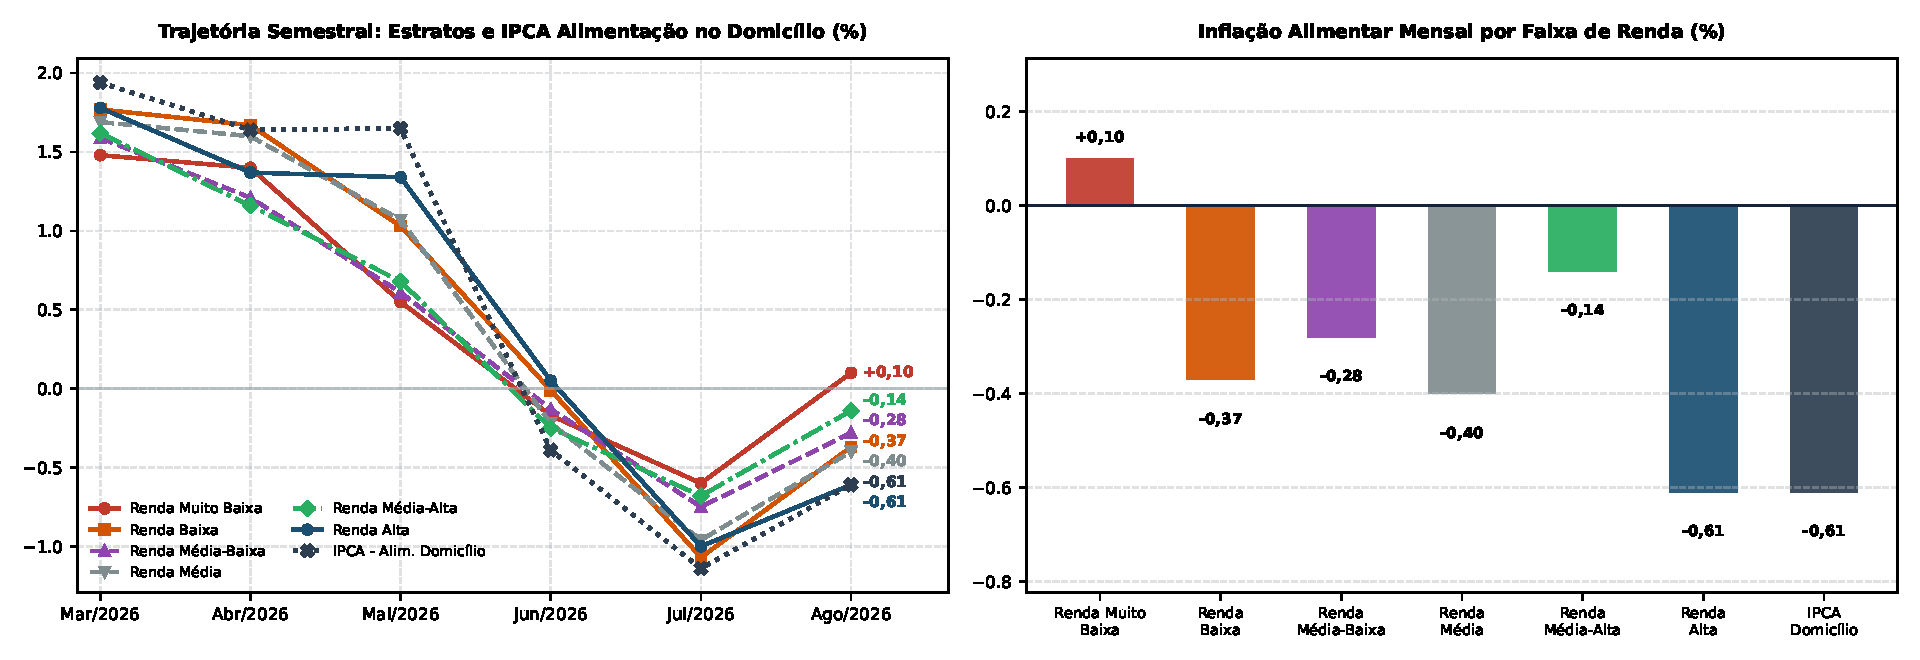
\includegraphics[width=\textwidth]{painel_1x2_trajetoria_barras.pdf}
		\vspace{2pt}
		\noindent\raggedright
		{\tiny \color{secondary} Fonte: Elaboração do autor com base em dados da POF 2017--2018 e Tabela 7060 (SIDRA/IBGE).}
	\end{figure}
	
	\clearpage
	
	% ==============================================================================
	% PÁGINA 3: O QUE EXPLICOU A VARIAÇÃO MENSAL E TABELA 1
	% ==============================================================================
	\cabecalhopadrao
	
	\noindent {\large \bfseries \color{bisnavy} O que Explicou a Variação Mensal}
	
	\vspace{0.06cm}
	
	{\small A Figura 2 mostra o que explica essa assimetria. O recuo em Frutas e Hortaliças atuou como a principal âncora deflacionária do mês, respondendo por contribuições de -0,62 p.p. na Renda Alta e -0,46 p.p. na Renda Média, frente a um efeito de apenas -0,03 p.p. na Renda Muito Baixa. Em contrapartida, o grupo de Proteínas Animais manteve pressão sobre o orçamento popular, adicionando +0,17 p.p. à taxa da Renda Muito Baixa e +0,21 p.p. à Renda Baixa. Os demais grupos apresentaram comportamento neutro a moderado.}
	
	\vspace{0.08cm}
	
	\begin{figure}[htbp]
		\centering
		\caption{Decomposição de contribuição (p.p.) por grupo de produtos nos seis estratos de renda.}
		\vspace{2pt}
		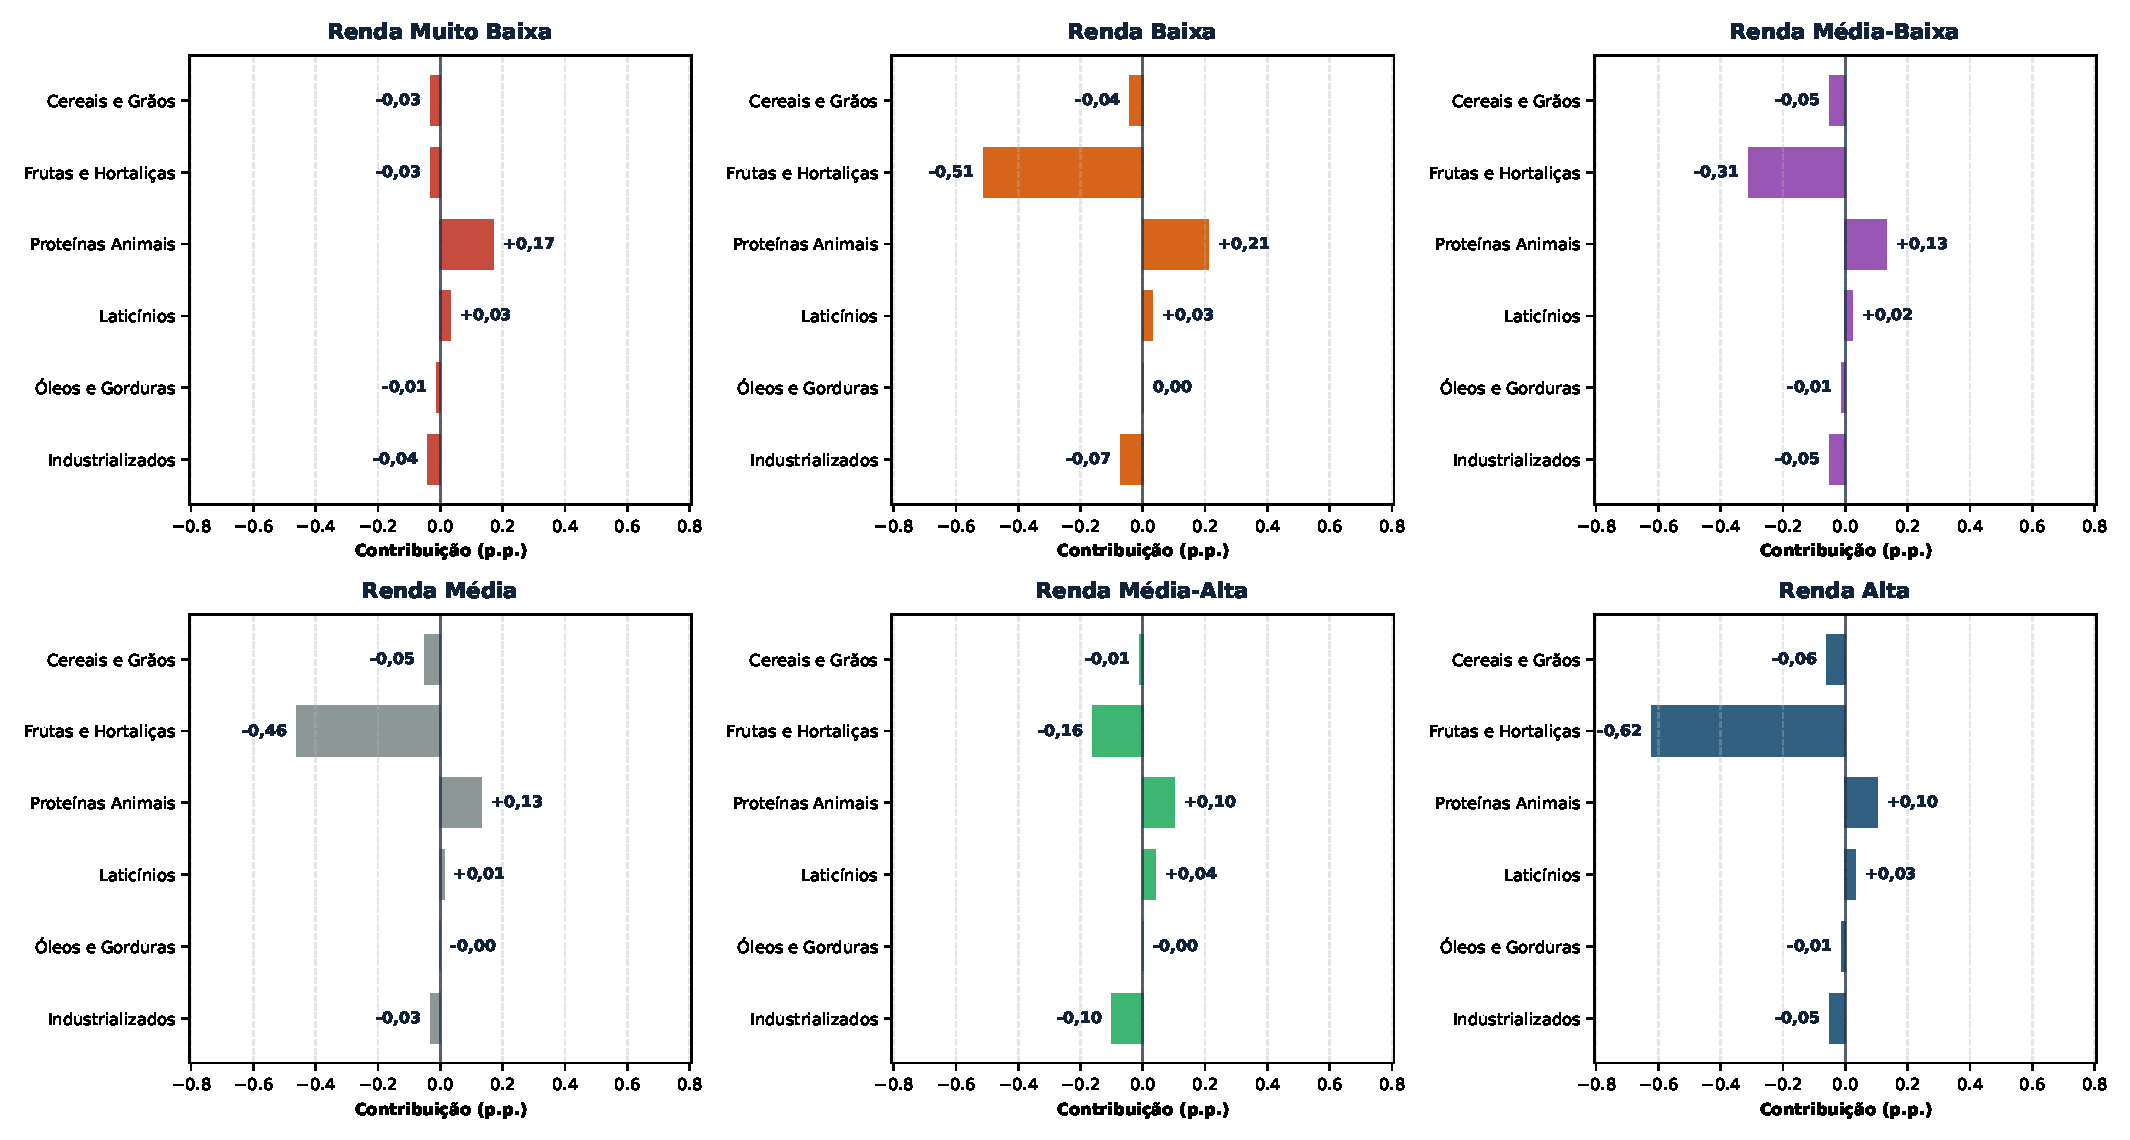
\includegraphics[width=0.96\textwidth]{painel_contribuicao_6faixas.pdf}
		\vspace{2pt}
		\noindent\raggedright
		{\tiny \color{secondary} Fonte: Elaboração do autor com base em dados da POF 2017--2018 e Tabela 7060 (SIDRA/IBGE).}
	\end{figure}
	
	\vspace{-0.15cm}
	
	\begin{table}[htbp]
		\centering
		\caption{Variação Mensal e Acumulada (\%)}
		\vspace{1pt}
		\footnotesize
		\begin{tabular*}{\textwidth}{@{\extracolsep{\fill}} l c c c c c @{}}
			\toprule
			& \multicolumn{3}{c}{\textbf{Variação Mensal}} & \multicolumn{2}{c}{\textbf{Variação Acumulada}} \\
			\cmidrule(lr){2-4} \cmidrule(lr){5-6}
			\textbf{Estrato / Indicador} & \textbf{Jun./26} & \textbf{Jul./26} & \textbf{Ago./26} & \textbf{12 Meses} & \textbf{No Ano} \\
			\midrule
			IPCA Geral & 0,16 & 0,07 & -0,32 & 4,22 & 3,11 \\
			IPCA - Alim. Domicílio & -0,39 & -1,14 & -0,61 & 2,77 & 3,42 \\
			\midrule
			
			Renda Muito Baixa & -0,17 & -0,60 & 0,10 & 4,34 & 3,87 \\
			
			Renda Baixa & -0,01 & -1,07 & -0,37 & 4,71 & 4,76 \\
			
			Renda Média-Baixa & -0,13 & -0,75 & -0,28 & 3,74 & 3,63 \\
			
			Renda Média & -0,22 & -0,96 & -0,40 & 4,75 & 4,17 \\
			
			Renda Média-Alta & -0,25 & -0,68 & -0,14 & 4,02 & 3,61 \\
			
			Renda Alta & 0,05 & -1,00 & -0,61 & 3,98 & 4,29 \\
			
			\bottomrule
		\end{tabular*}
		\vspace{2pt}
		\noindent\raggedright
		{\tiny \color{secondary} Fonte: Elaboração do autor com base na POF 2017--2018 e Tabela 7060 (SIDRA/IBGE). Padrão metodológico do Indicador Ipea de Inflação por Faixa de Renda aplicado à alimentação doméstica.}
	\end{table}
	
	\clearpage
	
	% ==============================================================================
	% PÁGINA 4: TABELA 2 (SUBITENS) EM PÁGINA DEDICADA INTEGRAL
	% ==============================================================================
	\cabecalhopadrao
	
	\noindent {\large \bfseries \color{bisnavy} Principais Contribuições Marginais de Subitens Alimentares por Estrato}
	\vspace{0.02cm}
	{\color{rulecolor}\hrule height 0.6pt}
	\vspace{0.06cm}
	
	{\small A tabela abaixo discrimina os cinco subitens que exerceram as maiores contribuições marginais positivas e negativas na formação da taxa mensal de cada estrato em Agosto de 2026.}
	
	\vspace{0.05cm}
	
	\begin{table}[htbp]
		\centering
		\caption{Principais Contribuições Marginais de Subitens Alimentares por Estrato (Agosto de 2026)}
		\vspace{2pt}
		\footnotesize
		\setlength{\tabcolsep}{4.5pt}
		\begin{tabular*}{\textwidth}{@{\extracolsep{\fill}} c l c c | l c c @{}}
			\toprule
			& \multicolumn{3}{c}{\textbf{Maiores Altas (+) por Contribuição}} & \multicolumn{3}{c}{\textbf{Maiores Quedas (-) por Contribuição}} \\
			\cmidrule(lr){2-4} \cmidrule(lr){5-7}
			\textbf{\#} & \textbf{Alimento} & \textbf{Var. (\%)} & \textbf{Contrib. (p.p.)} & \textbf{Alimento} & \textbf{Var. (\%)} & \textbf{Contrib. (p.p.)} \\
			\midrule
			
			\multicolumn{7}{l}{\textbf{\color{bisnavy}Renda Muito Baixa}} \\
			\midrule
			
			1 & Limão & +53,40 & +0,3580 & Couve-flor & -9,63 & -0,0904 \\
			
			2 & Maracujá & +19,22 & +0,1745 & Batata-inglesa & -19,89 & -0,0710 \\
			
			3 & Peixe - serra & +5,76 & +0,0498 & Açaí (emulsão) & -10,49 & -0,0603 \\
			
			4 & Pimentão & +6,24 & +0,0472 & Cenoura & -11,22 & -0,0592 \\
			
			5 & Carne de carneiro & +3,77 & +0,0361 & Pepino & -12,39 & -0,0567 \\
			
			\midrule
			
			\multicolumn{7}{l}{\textbf{\color{bisnavy}Renda Baixa}} \\
			\midrule
			
			1 & Limão & +53,40 & +0,1415 & Batata-inglesa & -19,89 & -0,1478 \\
			
			2 & Maracujá & +19,22 & +0,1265 & Pepino & -12,39 & -0,1238 \\
			
			3 & Peixe - serra & +5,76 & +0,0571 & Cenoura & -11,22 & -0,1110 \\
			
			4 & Peixe - palombeta & +3,13 & +0,0290 & Morango & -9,94 & -0,0827 \\
			
			5 & Banana-da-terra & +2,93 & +0,0280 & Açaí (emulsão) & -10,49 & -0,0729 \\
			
			\midrule
			
			\multicolumn{7}{l}{\textbf{\color{bisnavy}Renda Média-Baixa}} \\
			\midrule
			
			1 & Limão & +53,40 & +0,2834 & Pepino & -12,39 & -0,1014 \\
			
			2 & Maracujá & +19,22 & +0,0469 & Morango & -9,94 & -0,0940 \\
			
			3 & Pimentão & +6,24 & +0,0381 & Abobrinha & -8,88 & -0,0849 \\
			
			4 & Capa de filé & +3,66 & +0,0324 & Cebola & -11,07 & -0,0693 \\
			
			5 & Peixe - palombeta & +3,13 & +0,0313 & Cenoura & -11,22 & -0,0684 \\
			
			\midrule
			
			\multicolumn{7}{l}{\textbf{\color{bisnavy}Renda Média}} \\
			\midrule
			
			1 & Limão & +53,40 & +0,4922 & Cebola & -11,07 & -0,1166 \\
			
			2 & Maracujá & +19,22 & +0,0437 & Tomate & -10,94 & -0,1140 \\
			
			3 & Salame & +2,76 & +0,0289 & Morango & -9,94 & -0,1010 \\
			
			4 & Capa de filé & +3,66 & +0,0244 & Couve-flor & -9,63 & -0,0968 \\
			
			5 & Peixe - peroá & +2,58 & +0,0243 & Cenoura & -11,22 & -0,0895 \\
			
			\midrule
			
			\multicolumn{7}{l}{\textbf{\color{bisnavy}Renda Média-Alta}} \\
			\midrule
			
			1 & Limão & +53,40 & +0,4282 & Batata-inglesa & -19,89 & -0,1353 \\
			
			2 & Maracujá & +19,22 & +0,0852 & Couve-flor & -9,63 & -0,0975 \\
			
			3 & Banana-da-terra & +2,93 & +0,0320 & Açaí (emulsão) & -10,49 & -0,0932 \\
			
			4 & Peixe - sardinha & +2,75 & +0,0296 & Cebola & -11,07 & -0,0864 \\
			
			5 & Pimentão & +6,24 & +0,0279 & Cenoura & -11,22 & -0,0798 \\
			
			\midrule
			
			\multicolumn{7}{l}{\textbf{\color{bisnavy}Renda Alta}} \\
			\midrule
			
			1 & Limão & +53,40 & +0,1875 & Batata-inglesa & -19,89 & -0,2189 \\
			
			2 & Maracujá & +19,22 & +0,0509 & Pepino & -12,39 & -0,1231 \\
			
			3 & Peixe - serra & +5,76 & +0,0467 & Morango & -9,94 & -0,1014 \\
			
			4 & Pimentão & +6,24 & +0,0417 & Abobrinha & -8,88 & -0,0925 \\
			
			5 & Peixe - peroá & +2,58 & +0,0247 & Tomate & -10,94 & -0,0804 \\
			
			\midrule
			
			\bottomrule
		\end{tabular*}
		\vspace{3pt}
		\noindent\raggedright
		{\tiny \color{secondary} Fonte: Elaboração do autor com base na POF 2017--2018 e Tabela 7060 (SIDRA/IBGE). Nota: A ordenação é dada estritamente pela contribuição em pontos percentuais. A recorrência dos mesmos itens entre estratos decorre de a variação de preço ser uniforme nacionalmente; a diferenciação marginal advém estritamente do peso orçamentário relativo de cada produto na cesta familiar de cada faixa de renda.}
	\end{table}
	
	\clearpage
	
	% ==============================================================================
	% PÁGINA 5: FAIXAS DE RENDA, REPOSITÓRIO E NOTAS LEGAIS
	% ==============================================================================
	\cabecalhopadrao
	
	\noindent {\large \bfseries \color{bisnavy} Classificação Socioeconômica e Repositório Público}
	\vspace{0.02cm}
	{\color{rulecolor}\hrule height 0.6pt}
	\vspace{0.08cm}
	
	\noindent {\normalsize \bfseries \color{bisnavy} Estratificação Socioeconômica e Ponderação de Consumo}
	\vspace{0.06cm}
	
	{\small A classificação dos estratos adota a padronização oficial do Indicador Ipea de Inflação por Faixa de Renda, calibrada pela inflação acumulada e ancorada na POF 2017--2018.}
	
	\vspace{0.04cm}
	
	\begin{table}[htbp]
		\centering
		\caption{Faixas de Renda Mensal Domiciliar}
		\vspace{2pt}
		\footnotesize
		\begin{tabular*}{\textwidth}{@{\extracolsep{\fill}} l c c @{}}
			\toprule
			\textbf{Faixa de Renda} & \textbf{Renda Domiciliar (jan./2009)} & \textbf{Renda Domiciliar (jan./2026)} \\
			\midrule
			
			1 -- Renda muito baixa & Menor que R\$ 900,00 & Menor que R\$ 2.299,82 \\
			
			2 -- Renda baixa & De R\$ 900,00 a R\$ 1.350,00 & De R\$ 2.299,82 a R\$ 3.449,73 \\
			
			3 -- Renda média-baixa & De R\$ 1.350,01 a R\$ 2.250,00 & De R\$ 3.449,74 a R\$ 5.749,55 \\
			
			4 -- Renda média & De R\$ 2.250,01 a R\$ 4.500,00 & De R\$ 5.749,56 a R\$ 11.499,11 \\
			
			5 -- Renda média-alta & De R\$ 4.500,01 a R\$ 9.000,00 & De R\$ 11.499,12 a R\$ 22.998,22 \\
			
			6 -- Renda alta & Maior que R\$ 9.000,00 & Maior que R\$ 22.998,22 \\
			
			\bottomrule
		\end{tabular*}
		\vspace{2pt}
		\noindent\raggedright
		{\tiny \color{secondary} Fonte: Elaboração do autor com base na Carta de Conjuntura, Dimac/Ipea. \textbf{Nota Metodológica sobre o Enquadramento:} Os limites nominais apresentados para o ano corrente referem-se à calibragem fixada em jan./2026, calculada a partir do IPCA acumulado. A fixação no mês de janeiro estabelece uma régua de enquadramento estável para o acompanhamento ao longo de todo o ano de referência, evitando reclassificações artificiais das famílias mês a mês por variações inflacionárias transitórias.}
	\end{table}
	
	\vspace*{\fill}
	
	\noindent {\normalsize \bfseries \color{bisnavy} Acesso Direto à Base de Dados e Repositório Público}
	\vspace{0.06cm}
	
	{\small Para garantir transparência analítica e permitir auditoria independente, a série histórica completa cobrindo de Janeiro de 2020 a Agosto de 2026 --- acompanhada das matrizes de ponderação da POF 2017--2018, dos microdados dos subitens e da série de números-índice encadeados com base fixada em Janeiro de 2020 (\(= 100{,}00\)) --- encontra-se disponibilizada em repositório público:}
	
	\vspace{0.06cm}
	
	\begin{tcolorbox}[downloadbox]
		\centering
		{\bfseries \color{bisnavy} Acesso Direto à Nota Técnica e Séries Históricas Completas}\\[2pt]
		{\footnotesize \color{secondary} Repositório Institucional de Dados (Série Jan/2020 a Agosto de 2026)}\\[5pt]
		
		{\small
			\textbf{Nota Técnica Metodológica (PDF):} \href{https://raw.githubusercontent.com/Itaiguara-Bezerra/itaiguara-bezerra.github.io/main/dados/Nota_Tecnica_IPCA_Alimentacao_No_Domicilio_Por_Estrato_Socioeconomico.pdf}{download direto}\\[4pt]
			\textbf{Série de variações mensais (\%):} \href{https://raw.githubusercontent.com/Itaiguara-Bezerra/itaiguara-bezerra.github.io/main/dados/inflacao_mensal_ipca_renda_08_2026.xlsx}{.xlsx} \quad\textbar\quad \href{https://raw.githubusercontent.com/Itaiguara-Bezerra/itaiguara-bezerra.github.io/main/dados/inflacao_mensal_ipca_renda_08_2026.csv}{.csv} \quad\textbar\quad \href{https://raw.githubusercontent.com/Itaiguara-Bezerra/itaiguara-bezerra.github.io/main/dados/inflacao_mensal_ipca_renda_08_2026.parquet}{.parquet}\\[3pt]
			\textbf{Série de índices encadeados (Base 100 = Jan/2020):} \href{https://raw.githubusercontent.com/Itaiguara-Bezerra/itaiguara-bezerra.github.io/main/dados/indices_base100_ipca_renda_08_2026.xlsx}{.xlsx} \quad\textbar\quad \href{https://raw.githubusercontent.com/Itaiguara-Bezerra/itaiguara-bezerra.github.io/main/dados/indices_base100_ipca_renda_08_2026.csv}{.csv} \quad\textbar\quad \href{https://raw.githubusercontent.com/Itaiguara-Bezerra/itaiguara-bezerra.github.io/main/dados/indices_base100_ipca_renda_08_2026.parquet}{.parquet}
		}
	\end{tcolorbox}
	
	\vspace{0.10cm}
	
	\begin{tcolorbox}[notabox]
		{\bfseries \color{bisnavy} Nota de Isenção de Responsabilidade:}\\[2pt]
		{\footnotesize \color{secondary} As opiniões, análises e estimativas expressas neste relatório são de estrita e exclusiva responsabilidade do autor, não refletindo necessariamente a visão ou posicionamento oficial de quaisquer instituições com as quais mantenha vínculo profissional.}
	\end{tcolorbox}
	
	\vspace{0.08cm}
	
	% BLOCO COMO CITAR (PADRÃO RESEARCH CONSOLIDADO)
	\begin{tcolorbox}[notabox]
		{\bfseries \color{bisnavy} Como citar este documento:}\\[2pt]
		{\footnotesize \color{secondary} BEZERRA, Itaiguara de Oliveira. \textbf{Monitor da Inflação Alimentar: por Estrato de Renda}. Relatório de Acompanhamento Macroeconômico, Rio de Janeiro, Agosto de 2026. Metodologia de referência: BEZERRA, I. O. \textit{Mensuração da Inflação de Alimentação no Domicílio por Estrato Socioeconômico} (Nota Técnica, Outubro de 2026). É permitida a reprodução total ou parcial das informações, tabelas e metodologias aqui contidas, desde que expressamente citada a fonte e atribuída a autoria. Reproduções para fins comerciais são proibidas.}
	\end{tcolorbox}
	
	\vspace{0.10cm}
	{\color{rulecolor}\hrule height 0.5pt}
	\vspace{2pt}
	{\tiny \color{secondary} Relatório técnico independente. Fontes dos dados brutos: IBGE (POF / SIDRA).}
	
\end{document}